\documentclass{beamer}
\usepackage[orientation=portrait,size=a0,scale=1.4,debug]{beamerposter}
\mode<presentation>{\usetheme{W3F}}
\usepackage{chemformula}
\usepackage[utf8]{inputenc}
\usepackage[german, english]{babel} % required for rendering German special characters
\usepackage{siunitx} %pretty measurement unit rendering
\usepackage{hyperref} %enable hyperlink for urls
\usepackage{ragged2e}
\usepackage[font=scriptsize,justification=justified]{caption}
\usepackage{array,booktabs,tabularx}

\graphicspath{{figures/}}

\newcolumntype{Z}{>{\centering\arraybackslash}X} % centered tabularx columns
\sisetup{per=frac,fraction=sfrac}

\title{\huge Assessing or incentivising correct mixing \\ without centralised authorities}
\author{Jeffrey Burdges}
\institute[Web 3 Foundation]{Web 3.0 Foundation}
\date[Feb 2020]{Feb 2020}

% edit this depending on how tall your header is. We should make this scaling automatic :-/
\newlength{\columnheight}
\setlength{\columnheight}{104cm}


%%%%%%%%%%%%%%%%%%%%%%%%%%%%%%%%%%%%%%%%%%%%%%%%%%%%%%%%%%%%%%%%%%%%%%%%%%%%%%%%%%%%%%
\begin{document}
\begin{frame}
  \begin{columns}
    % ---------------------------------------------------------%
    % Set up a column 
    \begin{column}{.49\textwidth}
      \begin{beamercolorbox}[center,wd=\textwidth]{postercolumn}
        \begin{minipage}[T]{.95\textwidth}  % tweaks the width, makes a new \textwidth
          \parbox[t][\columnheight]{\textwidth}{ % must be some better way to set the the height, width and textwidth simultaneously
            % Since all columns are the same length, it is all nice and tidy.  You have to get the height empirically
            % ---------------------------------------------------------%
            % fill each column with content            
            \begin{block}{Assessment problem}
                Anonymity systems {\em assess} routers for performance, capacity, and reliability, \\ % \hspace*{3pt} 
                but do so using centralised infrastructure.  Can one decentralize assessment? \\  \bigskip\bigskip
                
                Example: Tor's bandwidth authority and special role flags. \\ \bigskip
            \end{block}
            \vfill
            \begin{block}{Rewards problem}
                Asking payments from users reduces the user base, aka anonymity set. \\ \bigskip
                Can one ``pay'' relays securely and efficiently? And avoid billing users? \\ \bigskip
            \end{block}
            \vfill
            \begin{block}{Bootstrap problem}
                Any cybercoin needs an initial or ongoing coin distribution scheme.  \\ \bigskip
                How can proof-of-stake cybercoins reward unstaked nodes? \\ \bigskip
            \end{block}
            \vskip1ex
            \vfill
            \begin{block}{Mix networks} % {Metadata protection}
                \hspace*{5pt} {\it ``[Tor does not] protect against an attacker who can see .. both \\
                \hspace*{5pt} traffic going into [and] coming out of the Tor network .. as \\
                \hspace*{5pt} simple statistics let you decide whether [both flows] match up.''} % \\
                \begin{columns}
                \begin{column}{.04\textwidth}
                \end{column}
                \begin{column}{.60\textwidth}
                \hspace*{30pt} \normalfont --Roger Dingledine, ``One cell is enough ..'' \\ \bigskip\bigskip\bigskip

                Among known ``anonymous'' messaging strategies, non-verifiable mix networks provide the least expensive and most scalable alternative, but..
                \end{column}
                \begin{column}{.45\textwidth}
                \begin{center}
                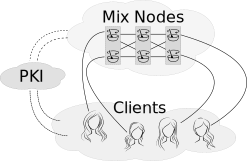
\includegraphics[width=0.75\textwidth]{../talks/pics/mix/initial} % was width=0.85
                \end{center}
                \end{column}
                \end{columns}                
                \bigskip

                \begin{itemize}
                \item 
                Mixnets incur latency due to a mixing strategy. \\
                We cannot adapt legacy protocols like HTTP to this higher latency, but.. \\
                we can design new protocols around the higher latency.
                \item 
                Mixnets require cover traffic (see Anonymity Trilemma \cite{anonymity_trilemma}) % \\
                \end{itemize}
                \bigskip
            \end{block}
            \vfill
            \begin{block}{Mixing strategy}
                We favor Poison or Stop-and-Go mixing where senders set packet delays obeying a memoryless exponential or geometric distribution, which defeats many active attacks. 
                \\ \bigskip
            \end{block}
            \vfill
            \begin{block}{Cover traffic}
                We've blend several cover categories using memoryless property of
                geometric or exponential distributions, several go nowhere special, but.. \\ \bigskip\bigskip

                Users maintain incoming cover traffic by sending themselves loop messages. \\ \bigskip\bigskip
                % , which \\ hides their real incoming messages.

                In Loopix \cite{Loopix}, mix nodes send themselves loop cover traffic too, which \\
                \begin{itemize}
                \item reduces adversaries' gains from monitoring mixes \cite[\S4.1.3: Thm 1 vs 2]{Loopix}, % and % see Theorem 1 vs 2 in \S4.1.3 of \cite{Loopix}.
                \item enable defenses against active attacks like n-1 attacks \cite[\S4.2.1]{Loopix}.
                \end{itemize}

                \begin{center}
                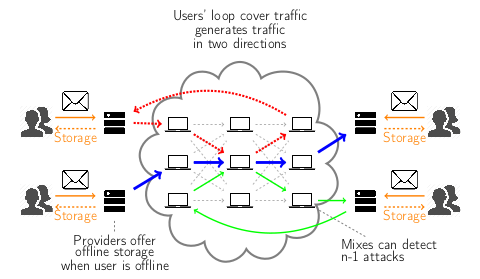
\includegraphics[trim=0 0 0 50,clip,width=\textwidth]{../talks/pics/loopix/achitecture}
                \end{center}

            \end{block}
            \vfill
            \begin{block}{VRFs}
                A {\em verifiable random function} (VRF) family is a pseudo-random function family parameterized by public-secret key pairs such that: \\
                \begin{itemize}
                \item  computing the function and proof requires the secret key, but
                \item  verifying correctness requires only the public key and proof.
                \end{itemize}
                \bigskip
            \end{block}
          }
        \end{minipage}
      \end{beamercolorbox}
    \end{column}
    % ---------------------------------------------------------%
    % end the column

    % ---------------------------------------------------------%
    % Set up a column 
    \begin{column}{.49\textwidth}
      \begin{beamercolorbox}[center,wd=\textwidth]{postercolumn}
        \begin{minipage}[T]{.95\textwidth} % tweaks the width, makes a new \textwidth
          \parbox[t][\columnheight]{\textwidth}{ % must be some better way to set the the height, width and textwidth simultaneously
            % Since all columns are the same length, it is all nice and tidy.  You have to get the height empirically
            % ---------------------------------------------------------%
            % fill each column with content

            \begin{block}{Assumptions}
                Mix network providing:
                \begin{enumerate}
                \item[1.] Shared global relay PKI or \dots \\ \bigskip 
                \item[2.] Loop cover packets sent by mixes.
                \end{enumerate}
                \bigskip
                Blockchain providing:
                \begin{enumerate}
                \item[3.] Some mix nodes have stake in some limited resource, but not all, \\ and
              non-transferable resources work, ala proof-of-personhood. \\ \bigskip
                \item[4.] All these staked nodes commit to VRF public keys $V = v G$. \\ \bigskip
                \item[5.] Some beacon that releases a shared random value $r_e$ in each epoch $e$.
                \end{enumerate}
            \end{block}
            \vfill
            \begin{block}{Protocol}
                Packet creation is deterministic given the seed, PKI, origin and destination. \\ \bigskip \bigskip

                Any staked mix $V$ sends cover packets $j < j_{\max}$ seeded by their VRF,
                \begin{center}
                $\rho_{V,e,j} := \mathtt{VRF}_v(r_e || j).\mathtt{Out}$
                \quad whenever \quad 
                $H_{\mathrm{send}}(\rho_{V,e,j}) < c'$. % {j_{\max} \over \lambda}
                \end{center}

                All mixes keep a replay protection database in any mix network, but \\
                after epoch $e$ our mixes commit to its state by publishing its merkle root. \\ \bigskip \bigskip

                After learning $r_{e+2}$ when epoch $e+2$ starts, each mix $V$ announces its \\
                VRF signature $\pi_{V,e,j}$ for exactly the $j$ for which $H(r_{e+2} \rho_{V,e,j}) < c$. \\ \bigskip \bigskip

                After seeing $\pi_{V,e,j}$, any node along the route taken by this packet either provides the mixing proof from its replay production database commitment, or else accuses its predecessors of dropping the packet.  \\ \bigskip
            \end{block}
            \vfill
            \begin{block}{Sampling}
                We blame whole routes for drops, never individual mixes, but.. \\ \bigskip
                We do produce a relatively random sample of the mix nodes' behavior, \\
                from which we accumulate rewards and report reliability to clients. \\ \bigskip \bigskip

                We envision a binomial or hypergeometric distribution for
                dropped out of non-dropped packets at each node in an epoch, for which
                we compute the maximum likelihood estimator over several epochs. \\ \bigskip \bigskip

                Mixes could manipulate drops counts by not announcing their winning $\pi_{V,e,j}$, \\
                but doing so should costs $V$, and it need not harm users much. \\ \bigskip \bigskip

                Attackers could beneficially impact rewards by biasing $r_e$ and/or $r_{e+2}$. \\ \bigskip
                We limit adversarial bias with longest chain analysis techniques \cite{OuroborosPraos} ,
                which suffices for assessments, but still biases rewards. \\ \bigskip \bigskip

                VDFs avoid such bias, but at extreme development costs. 
                RandHerd-like threshold VRFs protocols for unbiassed randomness pose their own liveness or security challenges. \\ \bigskip
            \end{block}
            % \vfill
            % \begin{block}{Economics}
            %     We propose a statistical sampling procedure for mix networks that exploits their cover traffic characteristics.
            % \end{block}
            \vfill
            \begin{block}{Conclusions} % 
                We require nothing from clients in this protocol, which aids adoption. \\ \bigskip \bigskip

                Anonymity suffers from our sampling only by retroactively leaking mix fullness, but using VRFs prevents this being used adversarially. \\ \bigskip \bigskip

                % We only perform sampling from staked mixes, but.. \\ \bigskip
                We sample and reward mixes without requiring that they be staked, only that they become listed in our PKI somehow.  \\ \bigskip \bigskip

                In particular we address the bootstrap problem for proof-of-stake protocols. \\ \bigskip
            \end{block}
            \vfill
            \vfill
			\begin{myblock}{References}
				\footnotesize
				\bibliographystyle{abbrv}
				\bibliography{../mix,../pos}
			\end{myblock}\vfill
          }
          % ---------------------------------------------------------%
          % end the column
        \end{minipage}
      \end{beamercolorbox}
    \end{column}
    % ---------------------------------------------------------%
    % end the column
  \end{columns}
  % \vskip1ex
  %\tiny\hfill\textcolor{ta2gray}{Created with \LaTeX \texttt{beamerposter}  \url{http://www-i6.informatik.rwth-aachen.de/~dreuw/latexbeamerposter.php}}
  %\tiny\hfill{Created with \LaTeX \texttt{beamerposter}  \url{http://www-i6.informatik.rwth-aachen.de/~dreuw/latexbeamerposter.php} \hskip1em}
\end{frame}
\end{document}


%%%%%%%%%%%%%%%%%%%%%%%%%%%%%%%%%%%%%%%%%%%%%%%%%%%%%%%%%%%%%%%%%%%%%%%%%%%%%%%%%%%%%%%%%%%%%%%%%%%%
%%% Local Variables: 
%%% mode: latex
%%% TeX-PDF-mode: t
%%% End:
